\documentclass[a4wide,11pt]{article}
\usepackage{graphicx}
\usepackage{color}
\usepackage{hyperref}
%\usepackage{a4wide}
\usepackage[a4paper, top=2cm, bottom=2cm, left=2cm, right=2cm]{geometry}
\usepackage{amsbsy,amsmath,amsfonts,amssymb,amsthm,amstext,amscd,amsxtra,amsopn}
\usepackage[]{subfigure}
\graphicspath{{images/}}


\renewcommand{\[}{\begin{equation}}
\renewcommand{\]}{\end{equation}}

\renewcommand{\{}{\begin{eqnarray}}
\renewcommand{\}}{\end{eqnarray}}

\renewcommand{\vec}{\mathbf}

\usepackage[dvipsnames]{xcolor}
\newcommand{\code}{\colorbox{yellow}}

\usepackage{listings}

\date{}
\begin{document}

	
	
\section{Introduction}

\href{https://github.com/thanospol/DIRECTFN}{DIRECTFN} package is free software for the accurate and efficient evaluation of four-dimensional singular integrals arising in Galerkin Method of Moments surface integral 
equation formulations over conforming triangular or quadrilateral meshes.  The fully-numerical algorithms of DIRECTFN~\cite{Polimeridis2013} are suitable for the following applications: 

\begin{itemize}
\item Weakly and strongly singular kernels
\item Planar and curvilinear elements
\item Basis/testing functions of arbitrary order
\item Problem-specific Green's functions (e.g. expressed in spectral integral form)
\item From zero frequency to frequencies beyond microwaves
\item Spectral convergence to machine precision
\end{itemize}

In general case,  DIRECTFN library is intended to compute the following weakly ($I_{WS}$) and strongly ($I_{SS}$) singular integrals:	
\[
\label{I_const_tri}
I_{WS} = \int\limits_{E_P}\int\limits_{E_Q} G(\vec r, \vec r') dS' dS,
\] 

\[
\label{I_WS}
I_{WS}^{m,n} = \int\limits_{E_P} \vec g_m(\vec r) \cdot\int\limits_{E_Q}  G(\vec r, \vec r') \cdot\vec f'_n(\vec r') dS' dS,\\
\]
\[
\label{I_SS}
I_{SS}^{m,n} = \int\limits_{E_P} \vec g_m(\vec r) \cdot\int\limits_{E_Q} (\nabla G(\vec r, \vec r') \times \vec f'_n(\vec r')) dS' dS.
\]
Here $E_P$ and $E_Q$ are observation and source elements, i.e., two triangles or two quadrilaterals, which may coincide (self-term case), have a common edge (edge adjacent case) or a common vertex (vertex adjacent case); $\vec f_n(\vec r')$ are basis and $\vec g_m(\vec r)$ are testing functions; $G(\vec r,\vec r')$ by default is homogeneous Green's function: $G(\vec r, \vec r') = \frac{e^{-ik|\vec r - \vec r'|}}{4\pi|\vec r - \vec r'|}$. However, it can be replaced by any function of source $\vec r'$ and observation $\vec r$ points $K(\vec r, \vec r') \sim |\vec r - \vec r'|^{-p},\quad p = 1, 2$.

There are several different sets of basis and testing functions implemented in DIRECTFN, and they will be described later in details. 
\section{Download}
The source code of \href{https://github.com/thanospol/DIRECTFN}{DIRECTFN} is written in C++11 and can be downloaded from Github repository~\cite{DIRECTFN}. Also, mex plugins are available to provide a fast Matlab interface to this functionality. The repository is structured as follows:
\begin{itemize}
	\item
\texttt{./include}
folder contains headers of the library with declarations only.
\item \texttt{./src} folder contains source
files where all the templates are instantiated in corresponding files properly. So, in the client programs
one can use the templated classes which have been precompiled already. 
 \item \texttt{./lib} is the target path to store the static library, which can be further used, e.g. in Matlab interface, or python wrappers.
\item \texttt{./tests} directory contains some
initial examples of how to use the library in your own code. 
\item \texttt{./examples} folder contains the scripts to reproduce results, presented in papers~\cite{Tambova_EuCap2017} and ~\cite{Tambova2017}.
\end{itemize}
\section{Compilation}

The provided static library and examples can be compiled using \href{https://www.gnu.org/software/make/}{make} utility. Therefore, it requires Windows users to have some Linux-like environment, such as \href{https://www.cygwin.com/}{Cygwin} or \href{http://www.mingw.org/}{MinGW}. However,the other possible option is to use \href{https://msdn.microsoft.com/en-us/library/dd9y37ha.aspx}{nmake} utility from Visual Studio (see~\ref{nmake}) . For the compilation you should do the following steps:

\begin{itemize}
\item First, go to the \texttt{./settings} directory and create or copy-modify platform-specific file\\  $\texttt{Makefile.your\_cpu\_alias}$.
Here the \texttt{your\_cpu\_alias} is an alias for your system compiler (like intel, gcc620, clang or so). This alias is
just an abbreviation to distinguish different Makefiles and can be any name you like.

\item Next, define environment variable \texttt{CPU=your\_cpu\_alias}. It can be done by the command
\begin{verbatim}
$ export CPU=your_cpu_alias
\end{verbatim}
or by figuring out the CPU explicitly when compiling the code with make utility:
\begin{verbatim}
make CPU=your_cpu_alias
\end{verbatim}

\item  Add  the following lines to the end of \texttt{./settings/Makefile.in}: 
 \begin{verbatim}
 ifeq ($(CPU),your_cpu_alias)
 include $(MF_PREFIX)/Makefile.target
 endif
 \end{verbatim}
 
 \item Finally, go to the \texttt{./lib/unix} folder and type 
 \begin{verbatim}
$ make
\end{verbatim}
 
or 
\begin{verbatim}
$ make CPU=your_cpu_alias
  \end{verbatim}
 This command will compile the code and move the static library into the \texttt{./lib} folder.
 Default name for the library is \texttt{directfn} (thus, it will be compiled and 
 builded in the \texttt{libdirectfn.a} after compilation).
 You can change the name in \texttt{settings/Makefile.in} by defining
 \texttt{DIRECTFN\_LIB\_NAME} variable.
\end{itemize}
Once the library is builded, you may go to the \texttt{./tests} or \texttt{./examples} folders
to compile and run some examples.
\subsection*{Compilation with nmake from Visual Studio}
\label{nmake}

In order to able working with the \href{https://msdn.microsoft.com/en-us/library/dd9y37ha.aspx}{nmake} utility, we provide also special Makefiles for it, since the syntax is slightly different from the one that \href{https://www.gnu.org/software/make/}{make} uses. To compile the source code with nmake you should do the following simple steps:
\begin{itemize}
	\item 
	Run the \href{https://msdn.microsoft.com/en-us/library/ms229859(v=vs.110).aspx}{Developer Command Prompt for Visual Studio} and change the folder to where you have cloned the repository.
	\item 
	Go to the folder \texttt{./lib/win/} and build the static library  by typing
	\begin{verbatim}
	nmake
	\end{verbatim}
	\item
	To compile the examples run the \href{https://msdn.microsoft.com/en-us/library/ms229859(v=vs.110).aspx}{Developer Command Prompt for Visual Studio} or Visual Studio x86(x64) Native Tools, change the folder to \texttt{.examples/<Paper Name>/c++} and type
\begin{verbatim}
nmake -f Makefile_win
\end{verbatim}
\end{itemize}
\section{Examples}
The folder \texttt{./examples} in the repository contains the scripts to reproduce results, presented in~\cite{Tambova_EuCap2017} and \cite{Tambova2017}. For a given example there are two ways to execute it:\\
\begin{itemize}
	\item 
	Go to \texttt{./examples/<Paper name>/c++/} folder and compile the C++ code by 
	\begin{verbatim}
	make
	\end{verbatim}
	or
	\begin{verbatim}
	nmake -f Makefile_win
	\end{verbatim}
	if you use Windows utility \texttt{nmake}.
	then type the name of the executable file
	\begin{verbatim}
	./test_name
	\end{verbatim}
	or just
	\begin{verbatim}
	test_name
	\end{verbatim} while using Visual Studio command prompt.
	It will create a file \texttt{Results$\_$<test$\_$name>.txt} with timings and errors, and you can open \texttt{Examples.ipynb} notebook and visualize the results by executing the corresponding cell. Note that to run the .ipynb file you need ipython to be installed.
	\item
	The other way is to use Matlab scripts. To do this, you first need to build the mex interface to C++ functions by going to the \texttt{./mex} folder and executing the \texttt{build.m} script. After that, you can switch to the folder \\
	\texttt{./examples/EuCap2017\_Examples/matlab} or \texttt{./examples/Full\_Paper\_Examples/matlab} and run any \texttt{test$\_$name.m} script and it will do all the computations and produce the error plots and timings automatically.
	\item
	Note that if you're going to build mex files with one of the standart Windows compiler, e.g., provided by Visual Studio, you should build the static library with Windows compiler as well, i.e., using nmake.
\end{itemize}
\section{Library Usage}
\subsection{Basic algorithm} 
\label{subs:libuse}
The complete manual of how to use DIRECTFN library can be found in \texttt{./docs/Manual}. Here we briefly describe the main steps of computing the surface-surface singular integrals. 
In C++, you first
\begin{verbatim}
#include "directfn_quad.h"
\end{verbatim}
 if you need to work with quadrilateral elements, or
\begin{verbatim}
#include "directfn_triag.h"
 \end{verbatim}
 if you need to work with triangles. Then you should define a "singular contour" \texttt{SingularContour3xn} according to adjacency type with the proper number of points:
\begin{verbatim}
SingularContour3xn cntr;
cntr.set_points(r1, r2, r3, r4);
\end{verbatim}
Here \texttt{double[3] ri} are coordinates of vertices of the considered elements in 3D--space.
 Note that the order of vertices for each case of adjacency must correspond to the rules defined below in  Sect.~\ref{Quadrilaterals} for quadrilaterals and Sect.~\ref{Triangles} for triangles. \\
 Next, create an object of \texttt{Quadrilateral$\_$ST(EA,VA)} algorithm () and use its interface instantiated by a \texttt{ParticularKernel} kernel type. 
\begin{verbatim}
unique_ptr<Quadrilateral_ST<ParticularKernel>> 
        up_quad_st(new Quadrilateral_ST<ParticularKernel>());
\end{verbatim}
The type \texttt{ParticularKernel}
is a C++ type which inherits the \texttt{AbstractKernel} class defined in \texttt{directfn\_kernel\_base.h/cpp}. Here and next we denote as "Kernel" all specific kernels implemented for quadrilaterals and triangles are discussed in details in the next sections.\\
Now you should define the wavenumber $\texttt{k0}$ and the orders of Gauss-Legendre quadratures\\ $\texttt{N1, N2, N3, N4}$, and assign your contour \texttt{cntr} with vertices to your object \texttt{up\_quad\_st}.
\begin{verbatim}
up_quad_st.set_wavenumber(k0);
up_quad_st.set_Gaussian_orders_4(N1, N2, N3, N4);
up_quad_st.set(cntr);
\end{verbatim}
Now you are ready to calculate the surface-surface singular integral(s) by calling
\begin{verbatim}
up_quad_st.calc_Iss(); // Iss = Integral Surface-Surface
\end{verbatim}
and use the obtained values.
\begin{verbatim}
const dcomplex * ref_val = up_quad_st->Iss();
// use ref_val somewhere
\end{verbatim}

If you need to recalculate these integrals for several contours or wave numbers we
strongly recommend to do it as it is shown above: create an object of the
\texttt{Quadrilateral\_ST(EA,VA)} algorithm once and then use it for contour points or other parameters
reset. This helps to avoid time-consuming memory allocation/deallocation related to creating and destroying the object.

In case you need to compute the integral once,
you can use more simple interface 
mostly developed for usage inside the Matlab scripts. ( See Sect.~\ref{matlab} and file \texttt{directfn\_quad.h}). 


\section{Quadrilateral elements}
\label{Quadrilaterals}
This section contains instructions how to use DIRECTFN to compute singular integrals over quadrilaterals. All the examples can be found in the repository in folder \texttt{./tests/basic}. The corresponding source files are \texttt{test$\_$directfn$\_$quad$\_$st.cpp}, \texttt{test$\_$directfn$\_$quad$\_$ea.cpp} and \\\texttt{test$\_$directfn$\_$quad$\_$va.cpp} for self-term(ST), edge adjacent (EA) and vertex adjacent (VA) cases, respectively.
\subsection{Setting the points}
As it were mentioned in~\ref{subs:libuse}, we first need to set the points of a "singular contour" \texttt{SingularContour3xn}. There are two types of quadrilateral elements, implemented in DIRECTFN: the four-node flat or bilinear quadrilaterals and nine-node quadratic quadrilaterals~\cite{Kolundzija_book}. Therefore, for the first type you need to specify:
\begin{itemize}
	\item 
	4 points for self-term case:
	\begin{verbatim}
	cntrST.set_points(r1, r2, r3, r4);
	\end{verbatim} 
	\item\
	6 points for edge-adjacent case:
	\begin{verbatim}
	cntrEA.set_points(r1, r2, r3, r4, r5, r6);
	\end{verbatim} 
	\item 
	7 points for vertex-adjacent case:
	\begin{verbatim}
	cntrVA.set_points(r1, r2, r3, r4, r5, r6, r7);
	\end{verbatim} 
\end{itemize}
In case of using curvilinear elements, you should specify:
\begin{itemize}
	\item 
	9 points for self-term case:
	\begin{verbatim}
	cntrST.set_points(r1, r2, r3, r4, r5, r6, r7, r8, r9);
	\end{verbatim} 
	\item\
	15 points for edge-adjacent case:
	\begin{verbatim}
	cntrEA.set_points(r1, r2, r3, r4, r5, r6, r7, r8, r9, r10,
	        r11, r12, r13, r14, r15);
	\end{verbatim} 
	\item 
	17 points for vertex-adjacent case:
	\begin{verbatim}
	cntrVA.set_points(r1, r2, r3, r4, r5, r6, r7, r8, r9, r10, 
	        r11, r12, r13, r14, r15, r16, r17);
	\end{verbatim} 
\end{itemize}
Note that the nodes of the associated quadrilaterals must follow the orientation depicted in Fig.\ref{fig:planar_quad_geom} for 4-node and Fig.\ref{fig:quad_curv_geom} for 9-node quadrilaterals.
\begin{figure}[h!]
	\subfigure{
\includegraphics[width = 0.22\linewidth]{ST_quad_geom}
		\label{fig:ST_quad_geom}}
	\hfill
	\subfigure{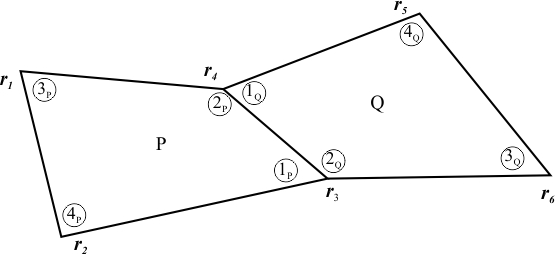
\includegraphics[width = 0.45\linewidth]{EA_quad_geom}
		\label{fig:EA_quad_geom}}
	\vfill\centering
	\subfigure{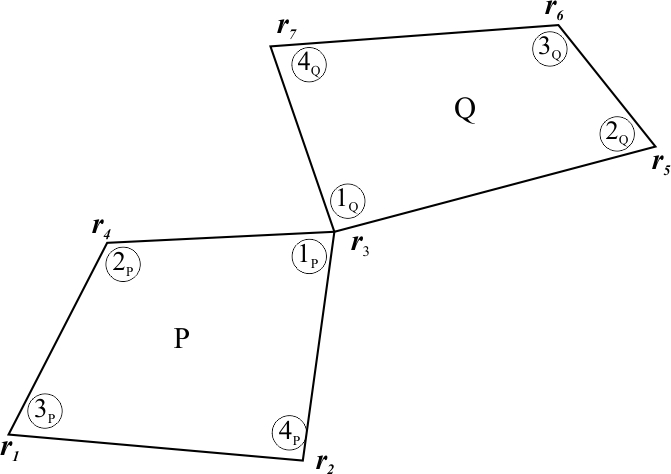
\includegraphics[width = 0.45\linewidth]{VA_quad_geom}
		\label{fig:VA_quad_geom}}
	\caption{Orientation of 4-node quadrilateral elements in DIRECTFN: \subref{fig:ST_quad_geom} self-term case \subref{fig:EA_quad_geom} edge adjacent case; \subref{fig:VA_quad_geom} vertex adjacent case.}
	\label{fig:planar_quad_geom}
\end{figure}
\begin{figure}
	\subfigure[]{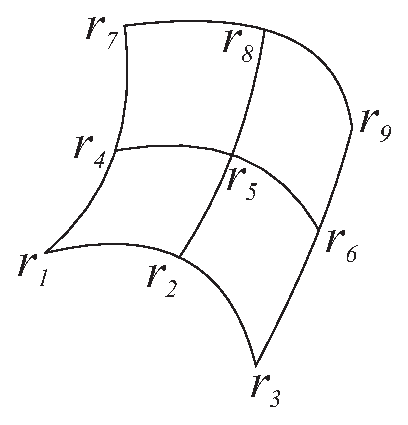
\includegraphics[width = 0.2\linewidth]{ST_curv_geom_quad}\label{fig:ST_geom_curv_quad}}
	\hfill
	\subfigure[]{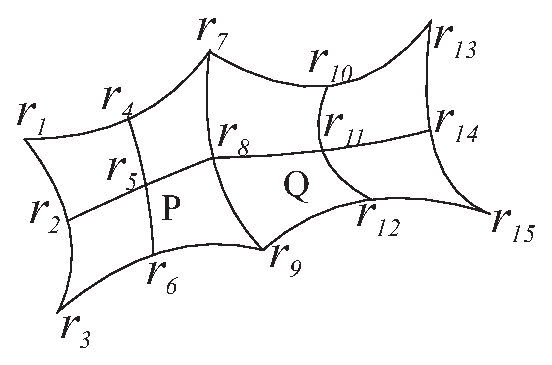
\includegraphics[width = 0.3\linewidth]{EA_curv_geom_quad}\label{fig:EA_geom_curv_quad}}
	\subfigure[]{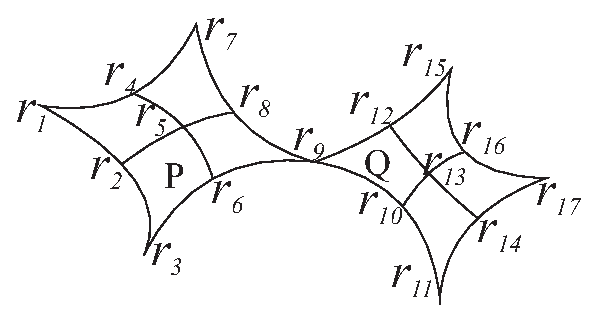
\includegraphics[width = 0.4\linewidth]{VA_curv_geom_quad}\label{fig:VA_geom_curv_quad}}
	\hfill
	\caption{Orientation of curvilinear quadrilateral elements in DIRECTFN:\subref{fig:ST_geom_curv_quad} self-term case; \subref{fig:EA_geom_curv_quad} edge adjacent case; \subref{fig:VA_geom_curv_quad} vertex adjacent case.}
	\label{fig:quad_curv_geom}
\end{figure}
\subsection{Choosing the basis and testing functions.}
\subsubsection*{Constant case}
The first and the simplest case implemented is the weakly singular integral with constant basis and testing functions:
\[
\label{I_const_quad}
I_{WS} = \int\limits_{E_P}\int\limits_{E_Q} G(\vec r, \vec r') dS' dS,
\] 
To compute this integral, after setting the contour, you should create an object of the ST,EA or VA algorithm \texttt{Quadrilateral$\_$ST(EA,VA)} with the type of the kernel \texttt{<QuadrilateralKernel$\_$PlanarScalar>}, if you work with planar elements
\begin{verbatim}
unique_ptr<Quadrilateral_ST<QuadrilateralKernel_PlanarScalar>> 
        up_quad_st(new Quadrilateral_ST<QuadrilateralKernel_PlanarScalar>());
\end{verbatim}
or with the kernel of the type \texttt{<QuadrilateralKernel$\_$CurvilinearScalar>}, if you use curvilinear elements:
\begin{verbatim}
unique_ptr<Quadrilateral_ST<QuadrilateralKernel_CurvilinearScalar>> 
        up_quad_st(new Quadrilateral_ST<QuadrilateralKernel_CurvilinearScalar>());
\end{verbatim}
\subsubsection*{Vector Basis and Testing Functions}
The other option is to compute the following weakly and strongly singular integrals:
\[
\label{I_WS}
I^{WS}_{m,n} = \int\limits_{E_P} \vec f_m(\vec r) \cdot\int\limits_{E_Q}  G(\vec r, \vec r') \cdot\vec f'_n(\vec r') dS' dS,\\
\]
\[
\label{I_SS}
I^{SS}_{m,n} = \int\limits_{E_P} \vec f_m(\vec r) \cdot\int\limits_{E_Q} (\nabla G(\vec r, \vec r') \times \vec f'_n(\vec r')) dS' dS,
\]
where $E_P$ and $E_Q$ are observation and source quadrilateral elements respectively, and $G(\vec r, \vec r') = \frac{e^{-ik|\vec r - \vec r'|}}{4\pi |\vec r - \vec r'|}$ is homogeneous Green's function.
Here $\vec f_m(\vec r )$ and $\vec f_n (\vec r'), (m,n = 1,2,3,4)$ are vector basis functions of the 1st order~\cite{Jin2014,Djordjevic2004}. For a given quadrilateral the four vector functions, associated with its edges are
\[
\label{vector_f}
\begin{aligned}
\vec b_1 &= (v-1)\frac{\vec r_v}{J(u,v)}, \quad \vec b_2 = (u+1)\frac{\vec r_u}{J(u,v)},\\
\vec b_3 &= (v+1)\frac{\vec r_v}{J(u,v)}, \quad \vec b_4 = (u-1)\frac{\vec r_u}{J(u,v)}.
\end{aligned},
\] 
where 
\[
\label{geom_Jacobian}
J(u,v) = |\vec r_u \times \vec r_v |,
\]
and 
\{
\label{derivatives}
\vec r_u \equiv \frac{\partial \vec r}{\partial u}= \frac {-\vec r_1 + \vec r_2 + \vec r_3 - \vec r_4 + v\left(\vec r_1 - \vec r_2 + \vec r_3 - \vec r_4\right)}4,\\
\vec r_v \equiv \frac{\partial \vec r}{\partial v} = \frac{-\vec r_1 - \vec r_2 + \vec r_3 + \vec r_4 + u\left(\vec r_1 - \vec r_2 + \vec r_3 - \vec r_4\right)}4.
\}
To compute these integrals over planar elements, you should create an object of the ST,EA or VA algorithm \texttt{Quadrilateral$\_$ST(EA,VA)} with the type of the kernel \texttt{<QuadrilateralKernel$\_$PlanarVectorWS>} for weakly singular integrals\eqref{I_WS}
\begin{verbatim}
unique_ptr<Quadrilateral_VA<QuadrilateralKernel_PlanarVectorWS>> 
       up_quad_va(new Quadrilateral_VA<QuadrilateralKernel_PlanarVectorWS>());
// WS = Weakly Singular
\end{verbatim}
and with the kernel of the type \texttt{<QuadrilateralKernel$\_$PlanarVectorSS>} for strongly singular integrals\eqref{I_SS}:
\begin{verbatim}
unique_ptr<Quadrilateral_EA<QuadrilateralKernel_PlanarVectorSS>> 
        up_quad_ea(new Quadrilateral_EA<QuadrilateralKernel_PlanarVectorSS>());
// SS = Strongly Singular
\end{verbatim}

For curvilinear elements the syntax is almost the same, 
\begin{verbatim}
unique_ptr<Quadrilateral_ST<QuadrilateralKernel_CurvilinearVectorWS>> 
        up_quad_st(new Quadrilateral_ST<QuadrilateralKernel_CurvilinearVectorWS>());
// WS = Weakly Singular
\end{verbatim}
for weakly singular integrals~\eqref{I_WS} and
\begin{verbatim}
unique_ptr<Quadrilateral_EA<QuadrilateralKernel_CurvilinearVectorSS>> 
        up_quad_ea(new Quadrilateral_EA<QuadrilateralKernel_CurvilinearVectorSS>());
// SS = Strongly Singular
\end{verbatim}
for strongly singular integrals~\eqref{I_SS}.
The output parameters for both cases are:
\[
\label{quad11}
\begin{matrix}
\begin{aligned}
I(1) \rightarrow I_{WS,SS}^{1,1}\\
I(2) \rightarrow I_{WS,SS}^{1,2}\\
I(3) \rightarrow I_{WS,SS}^{1,3}\\
I(4) \rightarrow I_{WS,SS}^{1,4}\\
I(5) \rightarrow I_{WS,SS}^{2,1}\\
I(6) \rightarrow I_{WS,SS}^{2,2}\\
I(7) \rightarrow I_{WS,SS}^{2,3}\\
I(8) \rightarrow I_{WS,SS}^{2,4}\\
\end{aligned}
&\quad\quad\quad &
\begin{aligned}
I(9) \rightarrow I_{WS,SS}^{3,1}\\
I(10) \rightarrow I_{WS,SS}^{3,2}\\
I(11) \rightarrow I_{WS,SS}^{3,3}\\
I(12) \rightarrow I_{WS,SS}^{3,4}\\
I(13) \rightarrow I_{WS,SS}^{4,1}\\
I(14) \rightarrow I_{WS,SS}^{4,2}\\
I(15) \rightarrow I_{WS,SS}^{4,3}\\
I(16) \rightarrow I_{WS,SS}^{4,4}\\
\end{aligned}
\end{matrix}
\]

\section{Triangular elements}
\label{Triangles}
This section contains instructions how to use DIRECTFN to compute singular integrals over triangular elements. All the examples can be found in the repository in folder \texttt{./tests/basic}. The corresponding source files are \texttt{test$\_$directfn$\_$triag$\_$st.cpp}, \texttt{test$\_$directfn$\_$triag$\_$ea.cpp} and \\\texttt{test$\_$directfn$\_$triag$\_$va.cpp} for self-term(ST), edge adjacent (EA) and vertex adjacent (VA) cases, respectively.
\subsection{Setting the points}
As for quadrilaterals, we first need to set the points of a "singular contour" \texttt{SingularContour3xn}. For the planar triangles, implemented in DIRECTFN, you should specify:
\begin{itemize}
	\item 
	3 points for self-term case:
	\begin{verbatim}
	cntrST.set_points(r1, r2, r3);
	\end{verbatim} 
	\item\
	4 points for edge-adjacent case:
	\begin{verbatim}
	cntrEA.set_points(r1, r2, r3, r4);
	\end{verbatim} 
	\item 
	5 points for vertex-adjacent case:
	\begin{verbatim}
	cntrVA.set_points(r1, r2, r3, r4, r5);
	\end{verbatim} 
\end{itemize}
Note that the nodes of the associated triangles must follow the orientation depicted in Figs~\ref{fig:EA_tri_geom} and~\ref{fig:VA_tri_geom}.
\begin{figure}[h!]
	\subfigure[]{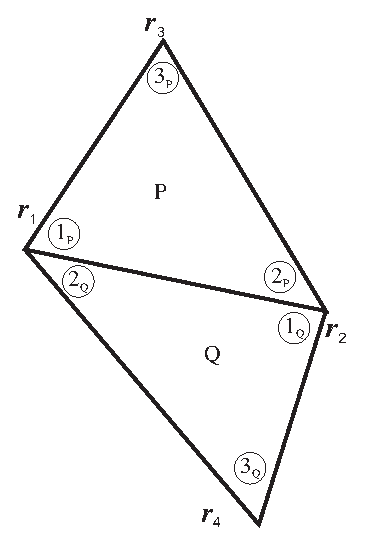
\includegraphics[width = 0.25\linewidth]{EA_tri_geom}
		\label{fig:EA_tri_geom}}
	\hfill
	\subfigure[]{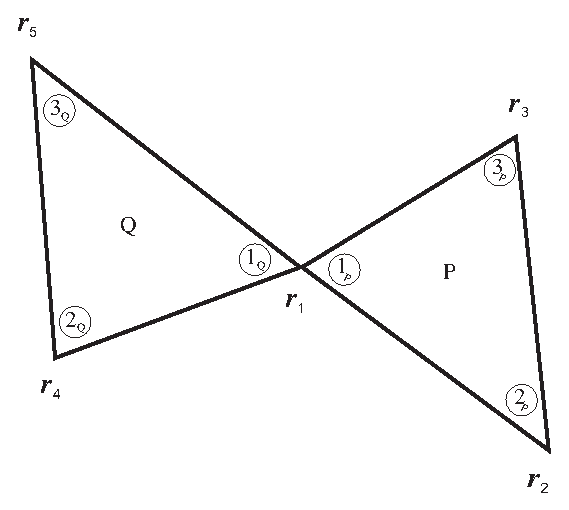
\includegraphics[width = 0.4\linewidth]{VA_tri_geom}
		\label{fig:VA_tri_geom}}
	\caption{Orientation of triangular elements in DIRECTFN: \subref{fig:EA_tri_geom} edge adjacent case; \subref{fig:VA_tri_geom} vertex adjacent case.}
	\label{tri_geom}
\end{figure}
\subsection{Choosing the basis and testing functions.}
\subsubsection*{Constant case}
To compute the weakly singular integral with constant basis and testing functions
\[
\label{I_const_tri}
I_{WS} = \int\limits_{E_P}\int\limits_{E_Q} G(\vec r, \vec r') dS' dS,
\] 
over trinagular elements, after setting the contour, you should create an object of the ST,EA or VA algorithm \texttt{Triangular$\_$ST(EA,VA)} with the type of the kernel \texttt{<TriangularKernel$\_$Constant$\_$ST(EA,VA)>}
\begin{verbatim}
unique_ptr<Triangular_ST<TriangularKernel_Constant_ST>> 
        up_tri_st(new Triangular_ST<TriangularKernel_Constant_ST>());
\end{verbatim}

\subsubsection*{Rao-Wilton-Glisson functions}

The other possible choice is to compute the following weakly and strongly singular integrals
\[
\label{I_WS_RWG}
I^{WS}_{m,n} = \int\limits_{E_P} \vec f_m(\vec r) \cdot\int\limits_{E_Q}  G(\vec r, \vec r') \cdot\vec f'_n(\vec r') dS' dS,
\]
\[
\label{I_SS_RWG}
I^{SS}_{m,n} = \int\limits_{E_P} \vec f_m(\vec r) \cdot\int\limits_{E_Q} (\nabla G(\vec r, \vec r') \times \vec f'_n(\vec r')) dS' dS,
\]
and
\[
\label{I_SS_nxRWG}
I^{SS}_{m,n} = \int\limits_{E_P} \left(\vec n(\vec r) \times\vec f_m(\vec r)\right) \cdot\int\limits_{E_Q} (\nabla G(\vec r, \vec r') \times \vec f'_n(\vec r')) dS' dS,
\]
where $E_P$ and $E_Q$ are observation and source flat triangular elements respectively, and $G(\vec r, \vec r') = \frac{e^{-ik|\vec r - \vec r'|}}{4\pi |\vec r - \vec r'|}$ is homogeneous Green's function. To compute these integrals, you should create an object of the ST, EA or VA algorithm \texttt{TriangularKernel$\_$ST(EA,VA)} with the types of the kernel: \\
\begin{itemize}
\item       
\texttt{<TriangularKernel$\_$RWG$\_$WS>} for weakly singular integral~\eqref{I_WS_RWG}
\begin{verbatim}
unique_ptr<Triangular_ST<TriangularKernel_RWG_WS>> 
        up_tri_st(new Triangular_ST<TriangularKernel_RWG_WS>());
\end{verbatim}
\item
\texttt{<TriangularKernel$\_$RWG$\_$SS>} for strongly singular integral~\eqref{I_SS_RWG}
\begin{verbatim}
unique_ptr<Triangular_EA<TriangularKernel_RWG_SS>> 
        up_tri_ea(new Triangular_EA<TriangularKernel_RWG_SS>());
\end{verbatim}
and
\item
\texttt{<TriangularKernel$\_$nxRWG$\_$SS>} for strongly singular integral~\eqref{I_SS_nxRWG}
\begin{verbatim}
unique_ptr<Triangular_VA<TriangularKernel_nxRWG_WS>> 
        up_tri_va(new Triangular_VA<TriangularKernel_nxRWG_SS>());
\end{verbatim}
\end{itemize}  

The output parameters for all the cases are:
\[
\label{tri16}
\begin{matrix}
\begin{aligned}
I(1) \rightarrow I_{WS,SS}^{1,1}\\
I(2) \rightarrow I_{WS,SS}^{1,2}\\
I(3) \rightarrow I_{WS,SS}^{1,3}\\
\end{aligned}
&
\begin{aligned}
I(4) \rightarrow I_{WS,SS}^{2,1}\\
I(5) \rightarrow I_{WS,SS}^{2,2}\\
I(6) \rightarrow I_{WS,SS}^{2,3}\\
\end{aligned}
&
\begin{aligned}
I(7) \rightarrow I_{WS,SS}^{3,1}\\
I(8) \rightarrow I_{WS,SS}^{3,2}\\
I(9) \rightarrow I_{WS,SS}^{3,3}\\
\end{aligned}
\end{matrix}
\]

\section{Matlab Interface}
\label{matlab}
We also provide a fast Matlab interface to have an easy access to DIRECTFN functionality.
The basic Matlab syntax to call the DIRECTFN procedures is
\begin{verbatim}
I = directfn_{quad,tri}_{st,ea,va}_{plan,curv}(r1,r2,...,N1,N2,N3,N4,ko,'BasisTestingType')
\end{verbatim}
Here the first several parameters \texttt{r1,r2,... }are positions of vertices. The required number and order of vertices is the same as in C++ and was considered earlier.
\texttt{N1,N2,N3,N4} are orders of Gaussian quadratures used in four 1-D integrals, \texttt{ko} is wavenumber.
The last parameter sets the type of basis and testing functions used. The possible values are:
\begin{itemize}
	\item \texttt{'Constant'} - for both quadrilaterals and triangles, standing for integrals~\eqref{I_const_quad} and~\eqref{I_const_tri},
	\item \texttt{'Vector$\_$WS'} and \texttt{'Vector$\_$SS'} - for quadrilaterals, computing the integrals~\eqref{I_WS} and~\eqref{I_SS}, and
	\item \texttt{'RWG$\_$WS'}, \texttt{'RWG$\_$SS'} and \texttt{'nxRWG$\_$SS'} for triangles, calculating the integrals~\eqref{I_WS_RWG},\eqref{I_SS_RWG}
 and \eqref{I_SS_nxRWG}.
\end{itemize} 

\section{Custom Kernels Implementation}
One remarkable property of our code design is that
integration algorithms are separated from the implementation of kernels to be integrated.
This means that anyone who wants to use his own particular kernel should implement
only the code related to the kernel and use the integration algorithms from the library by means of templates.
In this case he should also instantiate the templates by the kernel type like
\begin{verbatim}
template class Quadrilateral_ST<QuadrilateralKernel_PlanarScalar>;
\end{verbatim}	
or so. Search for the line "template class Quadrilateral" in all source files to find
all points of the instantiation of those types for your kernel.\\

If you need a kernel which depends on some parameters, you can call 
\texttt{kernel\_ptr()} of the integration algorithm class and then change the parameters 
of the kernel via its own interface (all data structures including kernels are allocated inside
the algorithms and uses smart pointers to avoid memory leaks).
\begin{verbatim}
ParticularKernel * const pkernel = quad_st.kernel_ptr();
for (double a = 0; a < 1.0; a += 0.1) {
    pkernel->reset_some_important_property(a);
    // computes integral with a changed
    quad_st.calc_Iss();   // Iss = Integral Surface-Surface
    const dcomplex * ref_val = up_quad_st->Iss();
    // use ref_val somewhere
}

\end{verbatim}
There are some other properties of algorithm classes. For details, please see 
\texttt{directfn\_interface.h/cpp} files.

The source code of DIRECFN library is structured as follows:

\begin{itemize}
\item \texttt{directfn\_interface.h/cpp}
is an abstract interface class. It provides  parameters setup  (number of points, singular
contour, etc) and obtaining the results of computation.

\item \texttt{directfn\_algorithm\_st.h/cpp}, \texttt{directfn\_algorithm\_ea.h/cpp},\\ 
and \texttt{directfn\_algorithm\_va.h/cpp} files contain integration algorithms  for self-term, edge-adjacent and vertex-adjacent cases
correspondingly for triangular and quadrilateral patches.

\item \texttt{directfn\_common.h/cpp} file contains some common routines, such as implementation of vector cross-product operation, or calculating normals. It includes auxiliary functions used throughout the \emph{algorithms}  implementation
(like computation of limits of integration, pointers to functions and all necessary common routines). 

\item \texttt{directfn\_gl\_1d.cpp} provides data for Gauss-Legendre integration points and weights.

\item \texttt{directfn\_arrsum.h/cpp} implements the classes responsible for vector summation of
internal subintegrals in \emph{algorithms}. They are especially useful for cases \eqref{quad11} and \eqref{tri16}.

\item \texttt{directfn\_contour.h/cpp}. Here the \texttt{SingularContour3xn} is implemented. It
provides the contour points setup and common interface to pass them inside classes of 
integration \emph{algorithms}.

\item \texttt{directfn\_kernel\_base.h/cpp} Contains base class for \emph{kernels} classes.
They are used in the integration \emph{algorithms}. Basically,
the methods
\begin{verbatim}
virtual void update_rp(const double uvxi_p[3]) noexcept = 0;
virtual void update_rq(const double uvxi_q[3]) noexcept = 0;
\end{verbatim}
are used to setup $\mathbf{r_p}$, $\mathbf{r_q}$ values and
 the method 
\begin{verbatim}
dcomplex value(const size_t index = 0) const noexcept;
\end{verbatim}
to compute it. The input argument \texttt{index} here exactly corresponds to the 
equations~\eqref{quad11}~and~\eqref{tri16}.
	
\item \texttt{directfn\_kernel\_quad\_geom.h/cpp} contains classes
responsible for planar and curvilinear geometry of quadrilateral elements.
	
\item \texttt{directfn\_kernel\_quad\_scal.h/cpp} contains kernels with constant basis/testing functions for quadrilaterals.

\item \texttt{directfn\_kernel\_quad\_vect.h/cpp} defines kernels with vector basis/testing functions for quadrilaterals.

\item \texttt{directfn\_kernel\_tri.h/cpp} defines kernels related to triangular elements (constant case, RWG basis functions).

\item \texttt{directfn\_greenfunc.h/cpp} implements the classes (base and derived ones) 
related to the  Green's functions, which are used inside the \emph{kernel} classes (as a pointer to a base virtual class).

\end{itemize}


\bibliography{IEEEabrv,References}
\bibliographystyle{IEEEtran}
\end{document}